\selectlanguage{english}
\settitle{Analyzing ARCompact Firmware with Ghidra}
\setauthor[N.~Iooss]{Nicolas Iooss\\
  \email{nicolas.iooss@ledger.fr}}
\institute{\raisebox{-0.2cm}{
\includegraphics[width=0.6cm]{AnalyzingARCompactFirmwareWithGhidra/img/donjon-black.pdf}} Ledger Donjon}

\setcounter{tocdepth}{2}  % show sections and subsections in PDF index

\ifdefined\pdftrailerid
  \pdftrailerid{} % For reproducible build
\fi

\maketitle
\index{Iooss, N.}

\begin{abstract}
Some microcontroller units use the ARCompact instruction set.
When analyzing their firmware, several tools exist to recover the code in assembly instructions.
Before this publication, no tool existed which enabled to recover the code in a language which is easier to understand, such as C language.

Ghidra is a powerful reverse-engineering project for which it is possible to add support for many instruction sets.
This article presents how ARCompact support was added to Ghidra and some challenges which were encountered in this journey.
This support enabled using Ghidra's decompiler to recover the semantics of the code of studied firmware in a language close to C.
\end{abstract}

\section{Introduction}

A modern computer embeds many microcontroller units (MCU). They are used
to implement complex features in the Network Interface Cards (NIC), the
hard disks, the flash memory devices, etc. These MCUs run code in a
similar way to usual processors: they use some \emph{firmware} which
contains instructions for a specific architecture.

For example:

\begin{itemize}

\item
  Some NICs implement complex features using MIPS instruction
  set~\cite{analyzingarcompactfirmwarewithghidra:sstic2010netcard}.
\item
  On some HP servers, the iLO (integrated Lights-Out) is implemented
  using ARM instruction
  set~\cite{analyzingarcompactfirmwarewithghidra:sstic2018ilo}.
\item
  On some Dell servers, the iDRAC (integrated Dell Remote Access
  Controller) is implemented using Renesas SuperH instruction
  set~\cite{analyzingarcompactfirmwarewithghidra:sstic2019idrackar}.
\item
  Some Hardware Security Modules (HSM) are implemented using PowerPC
  instruction
  set~\cite{analyzingarcompactfirmwarewithghidra:sstic2019hsm}.
\item
  On some Intel computers, the ME (Management Engine) is implemented
  using ARCompact instruction
  set~\cite{analyzingarcompactfirmwarewithghidra:recon2014intelme}.
\item
  On some of Lenovo's Thinkpad computers, the EC (Embedded Controller)
  is implemented using ARCompact instruction
  set~\cite{analyzingarcompactfirmwarewithghidra:thinkpadec,analyzingarcompactfirmwarewithghidra:sstic2011kbc}.
\item
  On some computers, the WiFi chipset runs code implemented using
  ARCompact instruction set (cf.~page 5
  of~\cite{analyzingarcompactfirmwarewithghidra:sstic2011kbc}).
\end{itemize}

Many of the used instruction sets have been implemented in
reverse-engineering tools such as \href{https://binary.ninja/}{Binary
Ninja}, \href{https://ghidra-sre.org/}{Ghidra},
\href{https://www.hex-rays.com/products/ida/}{IDA},
\href{https://github.com/jjyg/metasm}{metasm},
\href{https://github.com/cea-sec/miasm}{miasm},
\href{https://man7.org/linux/man-pages/man1/objdump.1.html}{objdump} and
\href{https://github.com/radareorg/radare2}{radare2}. However these
tools usually only implement a \emph{disassembler} for instructions sets
which are not widely used. The static analysis of firmware is much
easier when the code can be actually \emph{decompiled}, for example in C
language or in a pseudo-code which is easier to read than raw assembly
instructions.

\emph{Ghidra} (\url{https://ghidra-sre.org/}) is a powerful tool which
enables implementing a decompiler for any instruction set quite easily.
This relies on a domain-specific language called
SLEIGH~\cite{analyzingarcompactfirmwarewithghidra:ghidradoclanguage}.

\emph{ARCompact} is the name of an instruction set used by some ARC
processors (Argonaut RISC Core). It is still widely used in several MCUs
embedded in computers. This is why implementing support for this
instruction set in reverse-engineering tools can be very useful.

This article presents how the support for ARCompact was added to Ghidra
in order to analyze the firmware of an MCU studied by Ledger Donjon.
This support enabled using Ghidra's disassembler and decompiler in the
analysis. It was submitted as a Pull Request in May 2021,
\url{https://github.com/NationalSecurityAgency/ghidra/pull/3006}. This
article highlights the main challenges which were encountered and how
they were solved.

\section{ARCompact instruction set discovered through Ghidra}

When studying an instruction set, some characteristics need to be
determined. Is the length of instructions fixed? How many core registers
are available? Are there several address spaces for code and data? How
are functions called?

For ARCompact, the Programmer's
Reference~\cite{analyzingarcompactfirmwarewithghidra:arcompactisa}
provides answers to all these questions. ARCompact is an instruction set
which operates on 32-bit values using variable-length instructions.
There are sixty-four 32-bit core registers. Some instructions can be
conditionally executed, with a condition which depends on four condition
flags (\texttt{Z}, \texttt{N},
\texttt{C} and \texttt{V}) like ARM
instruction set\footnote{\texttt{Z} is the \emph{Zero}
  flag, \texttt{N} is the \emph{Negative} flag,
  \texttt{C} is the \emph{Carry} flag and
  \texttt{V} is the \emph{Overflow} flag.}. When
calling functions, the instruction \emph{Branch and Link}
(\texttt{bl}) puts the return address in the register
named \texttt{blink}, like ARM's link register.

These characteristics enabled to bootstrap ARCompact support in Ghidra.
For this, several files were created in a new directory named
\texttt{Ghidra/Processors/ARCompact} in Ghidra's
directory. These files were inspired from the support of other
instruction sets, including previous works about supporting
MeP~\cite{analyzingarcompactfirmwarewithghidra:beerump2019mep,analyzingarcompactfirmwarewithghidra:githubguedoumep,analyzingarcompactfirmwarewithghidra:githubxyzzmep}
and Xtensa instruction
sets~\cite{analyzingarcompactfirmwarewithghidra:githubyathxtensa,analyzingarcompactfirmwarewithghidra:githubprxtensa}.

The file which described how instructions are decoded,
\texttt{Ghidra/Processors/ARCompact/data/languages/ARCompact.slaspec}
was initialized with the definition of some registers
(listing~\ref{analyzingarcompactfirmwarewithghidra:regspec}).

\begin{lstlisting}[language=Python, numbers=left, caption={SLEIGH specification of ARCompact core registers}, label=analyzingarcompactfirmwarewithghidra:regspec]
define register offset=0x00 size=4 [
  r0 r1 r2 r3 r4 r5 r6 r7 r8 r9 r10 r11 r12 r13 r14 r15
  r16 r17 r18 r19 r20 r21 r22 r23 r24 r25 gp fp sp ilink1 ilink2 blink
  r32 r33 r34 r35 r36 r37 r38 r39 r40 r41 r42 r43 r44 r45 r46 r47
  r48 r49 r50 r51 r52 r53 r54 r55 r56 mlo mmid mhi lp_count r61reserved r62limm pcl
];
define register offset=0x130 size=1 [ Z N C V ];
\end{lstlisting}

Implementing the decoding of each instruction is then a matter of
defining \emph{tokens} to extract bits and defining the associated
semantics in pseudo-code. This process was described in length in
previous
presentations~\cite{analyzingarcompactfirmwarewithghidra:beerump2019mep}
and in Ghidra's
documentation~\cite{analyzingarcompactfirmwarewithghidra:ghidradoclanguage}.

There were several challenges in the implementation of ARCompact
instruction set. One of them was that instructions using 32-bits
constants encode them in a mix of Little Endian and Big Endian: the
value \texttt{0xAABBCCDD} is encoded as bytes
\texttt{BB AA DD CC}. This issue was solved by defining
a constructor \texttt{limm} (for \emph{long immediate})
using specific tokens
(listing~\ref{analyzingarcompactfirmwarewithghidra:limmspec}).

\begin{lstlisting}[language=Python, numbers=left, caption={SLEIGH specification of the decoding of 32-bit immediate values}, label=analyzingarcompactfirmwarewithghidra:limmspec]
define token limm_low_token (16) limm_low = (0, 15);
define token limm_high_token (16) limm_high = (0, 15);
limm: limm is limm_high ; limm_low [ limm = (limm_high << 16) + limm_low; ] { export *[const]:4 limm; }
\end{lstlisting}

Some other challenges are described in the following sections.

\section{64-bit multiplication}

The analyzed firmware contains the code in
listing~\ref{analyzingarcompactfirmwarewithghidra:mul64asm}.

\begin{lstlisting}[numbers=left, caption={Assembly code containing multiplication instructions}, label=analyzingarcompactfirmwarewithghidra:mul64asm]
Address  Bytes       Instruction        Description
c0085164 08 74       mov_s r12,r0     ; move the value in r0 to r12
c0085166 e0 78       nop_s            ; no operation
c0085168 1d 22 41 00 mpyu  r1,r2,r1   ; multiply r2 and r1 into r1
c008516c 1d 22 00 03 mpyu  r0,r2,r12  ; multiply r2 and r12 into r0
c0085170 1c 22 0b 03 mpyhu r11,r2,r12 ; multiply r2 and r12 and store the high 32 bits in r11
c0085174 1d 23 0c 03 mpyu  r12,r3,r12 ; multiply r3 and r12 into r12
c0085178 61 71       add_s r1,r1,r11  ; add r1 and r11 into r1
c008517a 99 61       add_s r1,r1,r12  ; add r1 and r12 into r1
c008517c e0 7e       j_s   blink      ; jump back to the caller
\end{lstlisting}

\texttt{mpyu} and \texttt{mpyhu}
compute the product of two 32-bit registers as a 64-bit value and store
in the destination register either the low 32 bits or the high 32 bits
of the result. Using both instruction could mean that the code
implements a 64-bit multiplication. When doing some maths, it appears
that the code indeed computes the 64-bit product of two 64-bit numbers.
With Ghidra, it is possible to accelerate this analysis by implementing
the semantics of the instructions.

The SLEIGH specification of these instructions was implemented as shown
in listing~\ref{analyzingarcompactfirmwarewithghidra:mul64spec}.

\begin{lstlisting}[language=Python, numbers=left, caption={SLEIGH specification of instructions \texttt{mpyu} and \texttt{mpyhu}}, label=analyzingarcompactfirmwarewithghidra:mul64spec]
:mpyhu^op4_dotcond op4_a, op4_b_src, op4_c_src is
  (l_major_opcode=0x04 & l_sub_opcode6=0x1c & l_flag=0 &
  op4_dotcond & op4_a) ... & op4_b_src & op4_c_src
{
  # extend source values to 64 bits
  local val_b:8 = zext(op4_b_src);
  local val_c:8 = zext(op4_c_src);
  # compute the product
  local result:8 = val_b * val_c;
  # extract high 32 bits
  op4_a = result(4);
}

:mpyu^op4_dotcond op4_a, op4_b_src, op4_c_src is
  (l_major_opcode=0x04 & l_sub_opcode6=0x1d & l_flag=0 &
  op4_dotcond & op4_a) ... & op4_b_src & op4_c_src
{
  local val_b:8 = zext(op4_b_src);
  local val_c:8 = zext(op4_c_src);
  local result:8 = val_b * val_c;
  # extract low 32 bits
  op4_a = result:4;
}
\end{lstlisting}

This enabled Ghidra to directly understand the function as the implementation of a 64-bit multiplication between values stored in registers \texttt{r1:r0} and \texttt{r3:r2} (figure~\ref{fig:analyzingarcompactfirmwarewithghidra:mul64} and listing~\ref{analyzingarcompactfirmwarewithghidra:mul64c}).

\begin{lstlisting}[language=C, numbers=left, caption={Decompiled output of the function given in listing~\ref{analyzingarcompactfirmwarewithghidra:mul64asm}}, label=analyzingarcompactfirmwarewithghidra:mul64c]
uint64_t mul64(uint64_t param_1,uint64_t param_2)
{
  return param_2 * param_1;
}
\end{lstlisting}

\begin{figure}[ht]
  \centering
  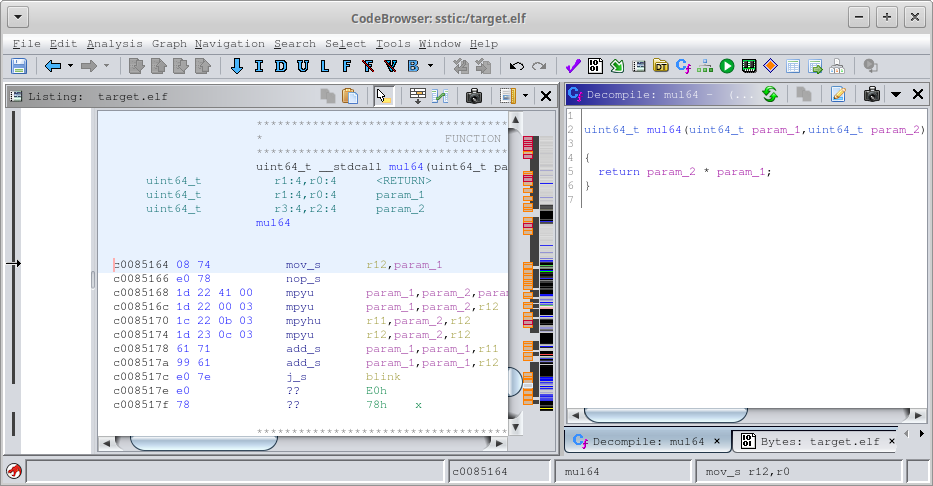
\includegraphics[width=\textwidth]{AnalyzingARCompactFirmwareWithGhidra/img/mul64}
  \caption{Implementation of a 64-bit multiplication}
  \label{fig:analyzingarcompactfirmwarewithghidra:mul64}
\end{figure}

This example shows how a decompiler can speed-up the time spent at
reverse-engineering a firmware. Instead of trying to understand how
\texttt{mpyu} and \texttt{mpyhu} are
combined together, it is possible to rely on the code produced by the
decompiler, which is much simpler.

\section{Loop instruction}

ARCompact instruction set provides an instruction named \emph{Loop Set
Up Branch Operation} and written \texttt{lp} in
assembly code. This instruction could be misleading. To understand it,
listing~\ref{analyzingarcompactfirmwarewithghidra:memcpyasm} presents a
piece of code which uses this instruction in the analyzed firmware.

\begin{lstlisting}[numbers=left, caption={Assembly code containing a loop}, label=analyzingarcompactfirmwarewithghidra:memcpyasm]
c0085230 0a 24 80 70     mov        lp_count,r2
c0085234 42 21 41 00     sub        r1,r1,0x1
c0085238 42 20 43 00     sub        r3,r0,0x1
c008523c a8 20 80 01     lp         LAB_c0085248

c0085240 01 11 84 02     ldb.a      r4,[r1,0x1]
c0085244 01 1b 0a 01     stb.a      r4,[r3,0x1]
                      LAB_c0085248
c0085248 20 20 c0 07     j          blink
\end{lstlisting}

Contrary to usual branching instruction,
\texttt{lp LAB\_c0085248} does not mean: branch to
address \texttt{c0085248} if some condition is met.
Instead, it means:

\begin{itemize}

\item
  Execute instructions until address \texttt{c0085248}
  is reached.
\item
  When reaching \texttt{c0085248}, decrement register
  \texttt{lp\_count}.
\item
  If \texttt{lp\_count} is not zero, branch back to the
  instruction right after \texttt{lp} (at address
  \texttt{c0085240}).
\end{itemize}

This makes the code repeat the instructions between
\texttt{lp} and the address given as parameter
(\texttt{c0085248}) exactly
\texttt{lp\_count} times. In this example, the
instructions copy a byte from the memory referenced by
\texttt{r1} into the one referenced by
\texttt{r3}, incrementing the pointers at each
iteration.

The problem caused by instruction \texttt{lp} is that
the semantic of the instruction located at the address given as
parameter changes. In order to decompile the example code correctly, the
semantic of the loop needs to be added to the instruction at address
\texttt{c0085248}.

In a real ARCompact MCU, \texttt{lp} is implemented by
using two auxiliary registers, \texttt{lp\_start} and
\texttt{lp\_end}:

\begin{itemize}

\item
  \texttt{lp LAB\_c0085248} puts the address of the
  next instruction (\texttt{c0085240}) into
  \texttt{lp\_start} and the given address
  \texttt{c0085248} into
  \texttt{lp\_end}.
\item
  When the MCU reaches address \texttt{c0085248}, as it
  matches the content of \texttt{lp\_end}, it
  decrements \texttt{lp\_count} and branches to
  \texttt{lp\_start} if it is not zero.
\end{itemize}

How such a semantic can be implemented in Ghidra? The answer is
surprisingly simple, thanks to Ghidra's documentation which already
contains an example of such a problem in
\url{https://ghidra.re/courses/languages/html/sleigh_context.html}:

\begin{quote}
\emph{However, for certain processors or software, the need to
distinguish between different interpretations of the same instruction
encoding, based on context, may be a crucial part of the disassembly and
analysis process.} {[}\ldots{]} \emph{For example, many processors
support hardware loop instructions that automatically cause the
following instructions to repeat without an explicit instruction causing
the branching and loop counting.}
\end{quote}

The SLEIGH processor specification language supports a feature called
\emph{context variables}. Here is how the \texttt{lp}
instruction was implemented with this feature.

First, a context was defined as well as a register storing
\texttt{lp\_start}
(listing~\ref{analyzingarcompactfirmwarewithghidra:loopspecctx}). Another
register was defined, \texttt{is\_in\_loop}, which
defines whether the \texttt{lp} instruction was
executed (which is important to implement conditional
\texttt{lp} instruction).

\begin{lstlisting}[language=Python, numbers=left, caption={SLEIGH specification of the context used to implement instruction \texttt{lp}}, label=analyzingarcompactfirmwarewithghidra:loopspecctx]
define register offset=0x140 size=4 [ lp_start ];
define register offset=0x148 size=1 [ is_in_loop ];
define register offset=0x200 size=4 [ contextreg ];

define context contextreg
  phase = (0,0)
  loopEnd = (1,1) noflow
;
\end{lstlisting}

Then, the decoding of \texttt{lp} sets the
\texttt{loopEnd} bit of the context to
\texttt{1} for the address given to
\texttt{lp}
(listing~\ref{analyzingarcompactfirmwarewithghidra:loopspeclp}). This is
done using a built-in function named
\texttt{globalset}.

\begin{lstlisting}[language=Python, numbers=left, caption={SLEIGH specification of instruction \texttt{lp}}, label=analyzingarcompactfirmwarewithghidra:loopspeclp]
:lp op4_lp_loop_end is
  l_major_opcode=0x04 & l_sub_opcode6=0x28 & l_flag=0 &
  l_op_format=2 & op4_lp_loop_end
  [ loopEnd = 1; globalset(op4_lp_loop_end, loopEnd); ]
{
  lp_start = inst_next;
  is_in_loop = 1;
}
\end{lstlisting}

Finally, to change the semantic of the instruction which ends the loop,
a two-phase instruction decoding was implemented
(listing~\ref{analyzingarcompactfirmwarewithghidra:loopspecphase}).

\begin{lstlisting}[language=Python, numbers=left, caption={SLEIGH specification of a two-phase instruction decoding pipeline}, label=analyzingarcompactfirmwarewithghidra:loopspecphase]
:^instruction is phase=0 & instruction
  [ phase = 1; ]
{
  build instruction;
}
:^instruction is phase=0 & loopEnd=1 & instruction
  [ phase = 1; ]
{
  if (is_in_loop == 0) goto <end_loop>;
  lp_count = lp_count - 1;
  if (lp_count == 0) goto <end_loop>;
  pc = lp_start;
  goto [pc];
<end_loop>
  is_in_loop = 0;
  build instruction;
}

with: phase = 1 {

# ... all instructions are decoded here

}
\end{lstlisting}

With these changes, the instructions of the example are decompiled as something which seems to be a correct implementation of a \texttt{memcpy} function (figure~\ref{fig:analyzingarcompactfirmwarewithghidra:memcpy} and listing~\ref{analyzingarcompactfirmwarewithghidra:loopc}).

\begin{lstlisting}[language=C, numbers=left, caption={Decompiled output of the instructions given in listing~\ref{analyzingarcompactfirmwarewithghidra:memcpyasm}}, label=analyzingarcompactfirmwarewithghidra:loopc]
  puVar3 = (undefined *)((int)src + -1);
  puVar4 = (undefined *)((int)dst + -1);
  do {
    puVar3 = puVar3 + 1;
    puVar4 = puVar4 + 1;
    *puVar4 = *puVar3;
    size = size - 1;
  } while (size != 0);
  return;
\end{lstlisting}

\begin{figure}[ht]
  \centering
  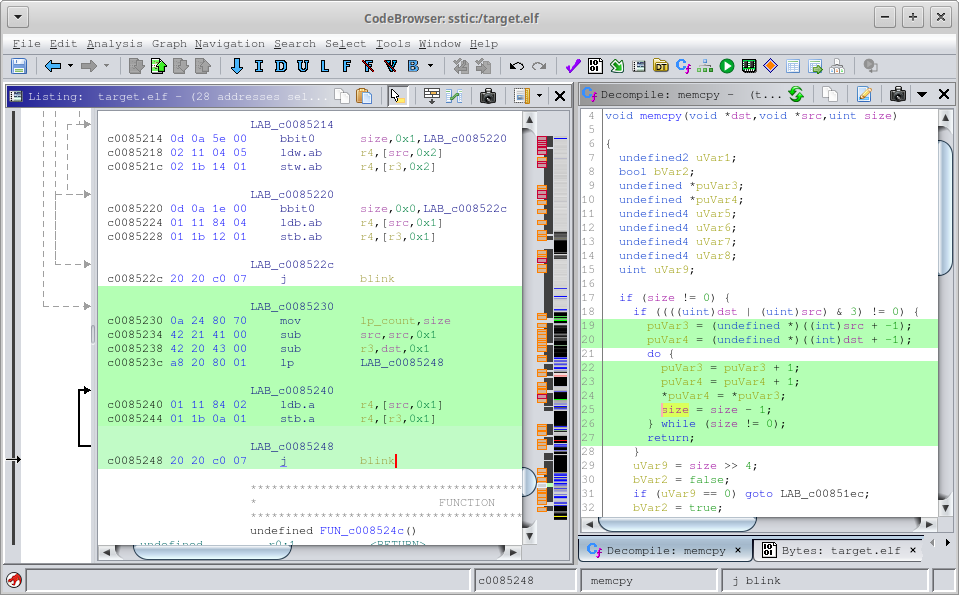
\includegraphics[width=\textwidth]{AnalyzingARCompactFirmwareWithGhidra/img/memcpy}
  \caption{Implementation of \texttt{memcpy} in the studied firmware}
  \label{fig:analyzingarcompactfirmwarewithghidra:memcpy}
\end{figure}

\section{Conclusion}

Thanks to this work, it is possible to perform static analysis on
firmware of some MCUs using ARCompact. This work enabled Ledger's
security team to bypass the secure boot feature of a MCU. This result
will hopefully be presented in the future. This will also help finding
issues in code running on MCUs, for example by plugging a fuzzer to
Ghidra's machine emulator.

\bibliography{AnalyzingARCompactFirmwareWithGhidra/biblio}
